\documentclass[10pt,table,dvipsnames]{beamer}
\usepackage{tikz}
\usepackage{mathptmx}
\usepackage[scaled=0.94]{helvet}
\usepackage[absolute,overlay]{textpos}
\usepackage{hyperref}
\usepackage{listings}
\lstloadlanguages{python}

\author{S.~Poss}
\title{ILCDIRAC}
\subtitle{A few words on future plans}
\date{Feb. 2, 2013}
\institute{CERN, LAPP}
\newcommand{\interstitial}[1]{\begin{frame}\begin{block}{}\centering\Huge{#1}\end{block} \end{frame}}
\newcommand{\backupslides}{\interstitial{Backup Slides}}

\mode<all>
\TPGrid{50}{50}

\pgfdeclareimage[width=0.1\paperwidth]{cliclogo}{CLIClogo}
\newcommand{\ClicLogo}{%
\begin{textblock}{14}(45., 0.05)
 \href{http://lcd.web.cern.ch}{\pgfuseimage{cliclogo}}
\end{textblock}
}

\setbeamertemplate{footline}
{%
  \leavevmode%
  \hbox{%
  \begin{beamercolorbox}[wd=.222222\paperwidth,ht=2.25ex,dp=1ex,left]{title in 
head/foot}%
    \usebeamerfont{date in head/foot}\insertshortdate{}\hspace*{2em}
  \end{beamercolorbox}%
  \begin{beamercolorbox}[wd=.555555\paperwidth,ht=2.25ex,dp=1ex,center]{author 
in head/foot}%
    \usebeamerfont{author in head/foot}\insertshortauthor{}:
    \usebeamerfont{title in head/foot}\insertshorttitle
  \end{beamercolorbox}%
  \begin{beamercolorbox}[wd=.222222\paperwidth,ht=2.25ex,dp=1ex,right]{date in 
head/foot}%
    \insertframenumber{}/\inserttotalframenumber\hspace*{2ex}
  \end{beamercolorbox}}%
  %\vskip0pt%
  \ClicLogo
}

\beamertemplatenavigationsymbolsempty
\setbeamertemplate{blocks}[rectangle]
\setbeamersize{text margin left=1em,text margin right=1em}

%\setbeamertemplate{headline}[default]

\begin{document}
\renewcommand{\inserttotalframenumber}{\ref{lastframe}}

\begin{frame}
\titlepage
\end{frame}

\begin{frame}
\frametitle{Outline}
\tableofcontents
\end{frame}

%\section{Introduction}\label{sec:intro}
%\begin{frame}
%  \frametitle{A few ideas}
%  \begin{itemize}
%  \item Whizard 2 support
%  \item File catalog 
%  \item Use case in DESY
%  \end{itemize}
%\end{frame}
%
\section{Whizard 2}
\label{sec:whiz2}
\begin{frame}
  \frametitle{Whizard 2 support: process factory?}
Idea:
\begin{itemize}
\item Propose a production service to users
\item WHIZARD 2 can take a process definition and provide a binary
\item Integrate this in the DIRAC production system (or interface to
  it)
\end{itemize}
\end{frame}
\begin{frame}
  \frametitle{What would be needed?}
  \begin{itemize}
  \item Web interface for fanciness, and CLI for gurus
  \item DIRAC service to listen to the queries
  \item Agent to run WHIZARD2 and produce the binary
  \item Agent to monitor everything
  \item Notification to notify the user about completion (already in DIRAC)
  \item Interface to DIRAC Transformation service to produce the
    events
  \item Some state machine
  \end{itemize}
\end{frame}
\begin{frame}
  \frametitle{Proposed interface}
What would be required from the user:
\begin{itemize}
\item Process definition (a la WHIZARD 2, in sindarin), also the
  Machine for lumi spectrum
\item Generator level cuts (if any), either in whizard or using the
  StdHepCut framework
  \begin{itemize}
  \item Will have to find a way to include user code easily (maybe
    include it in the whizard compilation procedure)
  \end{itemize}
\item Simulation parameters
  \begin{itemize}
  \item Detector model (sidloi3, ILD\_o1\_01,
  CLIC\_ILD\_CDR, etc.), 
  \item Steering files 
  \item Software version (detector type should be enough to get the
    software type: Mokka, SLIC, etc.)
  \end{itemize}
\item Reco parameters
  \begin{itemize}
  \item Steering files
  \item Software version: again, Marlin/LCSIM chain can be determined
    from detector model
  \item Adding overlay: need to add check of availability of
    background events for machine/detector/energy
  \end{itemize}
\end{itemize}
\end{frame}
\begin{frame}
\frametitle{How would it work?}
\begin{itemize}
  \item The service stores the process request: what has to be done,
  how, etc.\\
~\\
  \item Submission Agent picks up any New request, checks if the process is
  already there (implies clever look up in DB)
  \begin{itemize}
    \item If YES, then create transformation (or extend existing one,
    which needs storing also Transformation IDs),
    send notification to the user about the prod ID
    \item if NO: compile the whizard binary (with whizard2), compile
    cuts (svn up, compile),  add them as a software in the
    DIRAC CS, create the transformation, notify the user about
    TransformationID to monitor. 
    \item Notify the user in case of
    (compilation) failures
    \item Could use submitter credentials for the jobs
    \item Need a way to ``guess'' the time it takes to generate N
    events to maximize CPU efficiency
  \end{itemize}
\end{itemize}
\end{frame}

\begin{frame}
  \frametitle{How would it work?}
\begin{itemize}
  \item Monitoring Agent (on Running requests): 
  \begin{itemize}
    \item When number of events requested in given
     Request achieved, notify the user that the job is
     done, and give him the LFN directory or meta data query
     corresponding (by mail).
    \item Extend remaining productions to reach desired number of
     events: needs knowledge of current state
    \item Should be able to pick up cases when the CPU time per job is
     reached, and create splitting tasks as well as merging tasks
    \item Check failure rate and stop if threshold reached (+ notify user/admin)
  \end{itemize}
  \item Cleaning Agent (on Cleaning, deleted, etc):
  \begin{itemize}
    \item Remove the whizard binary from the GRID
    \item Issue the proper request to the Transformation System (Clean,
      Archive)
    \item Clean tables accordingly.
  \end{itemize}
\end{itemize}
Of course all those are ONLY ideas, most likely far from final product
\end{frame}

\section{File Catalog(s)}
\label{sec:fc}

\begin{frame}
  \frametitle{File catalog(s)}
Currently for replica:
\begin{itemize}
\item Lcg File Catalog: used for ILD DBD studies, being more or less
  dropped by the LHC experiements (lead dev retired). Fairly slow as
  usually the server is shared between multiple VOs
\item DIRAC File Catalog: Used for CLIC CDR and SID DBD, supported by
  the community. Quite fast as dedicated to only ILC (and CALICE)
\end{itemize}
~\\
For meta data:
\begin{itemize}
\item FC from DESY: used for ILD DBD, access with DJANGO interface,
  file level meta data
\item DFC again: used for CLIC CDR and SID DBD, file and directory
  meta data
\end{itemize}
Can interface the FC from DESY to use the replica catalog part of the
DFC instead of the LFC.
\end{frame}

\section{Conclusion}
\label{sec:conc}
\begin{frame}
  \frametitle{Conclusion}
\begin{block}{ILCDIRAC is:}
\begin{itemize}
\item A \alert{fully functionnal grid solution} for the Linear Collider
  community
  \begin{itemize}
  \item Used for {\color{ForestGreen}CLIC CDR} and {\color{ForestGreen}ILC DBD} activities\\~\\
  \end{itemize}
\item Coming with an {\color{NavyBlue}intuitive/user friendly} interface\\
~\\
\item {\color{NavyBlue}Easily connected with any new resources} (Site, storage,
  etc.)\\
~\\
\item {\color{NavyBlue}Open source}\\
~\\
\item {\color{NavyBlue}Available} for any ILC VO member
\end{itemize}
\end{block}
\label{lastframe}
\end{frame}

\backupslides

\begin{frame}
  \frametitle{Site usage}
\centering
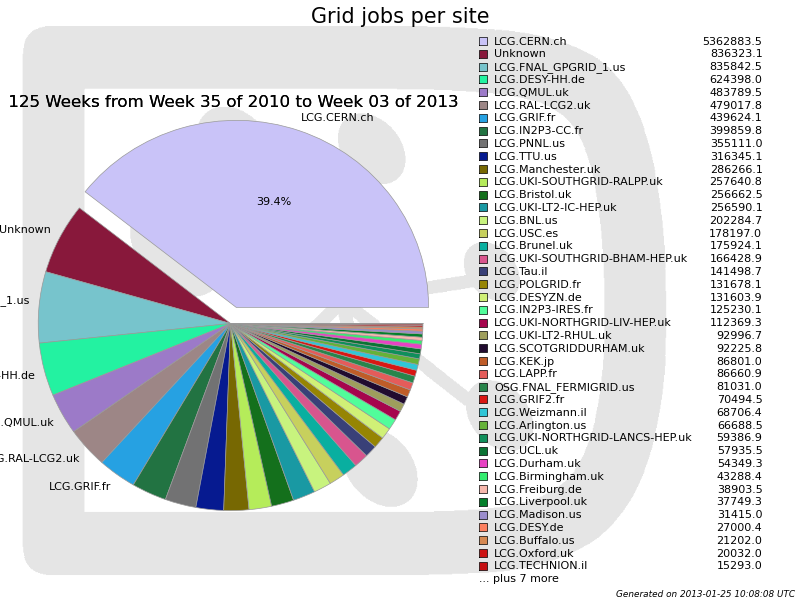
\includegraphics[width=0.9\textwidth]{PilotsPerSite}\\
\end{frame}
\end{document}


% Local Variables:
% TeX-PDF-mode: t
% End:
